
\section{Methodology}
\label{sec:method}

In this Section we discuss a Bayesian method for stellar photometric distance estimation and its implementation.
We start with a brief overview of Bayesian methodology and then discuss in detail our choices of likelihoods
and priors, and how they differ from previous work. A pipeline implementation of this method and a discussions
of its performance are presented in the next Section. 


\subsection{Bayesian Approach to Stellar Photometric Distance Estimation}

In most general terms, our aim is to estimate for each star an array (a vector) of model parameters $\vec{\theta}$,
for some model $M$ (e.g., main-sequence stars), using data vector $\vec{D}$ and priors for $M$ and $\vec{\theta}$.
Data, or observations, include multi-band photometry that is used
to construct colors, $\vec{c}$. In the case of SDSS, colors include $u-g$, $g-r$, $r-i$, $i-z$, and in the case of LSST also
$z-y$. In addition to colors, $\vec{D}$ also includes an apparent magnitude and hereafter we choose the $r$-band
magnitude. Therefore, $\vec{D}$ = ($r$, $\vec{c}$). Observations also provide stellar sky coordinates and we
address their role further below when discussing priors.

Models $M$ (either empirical or computational, see below) need to provide stellar colors as functions of model parameters
$\vec{\theta}$. 
The three principal parameters that control stellar colors at a fixed stellar age and at the accuracy level relevant here
($\sim$1 \%) include absolute magnitude (here chosen in the $r$ band, $M_r$), metallicity ($[Fe/H]$) and surface
gravity. In the case of main-sequence stars and red giants, the color tracks can be expressed as functions of $M_r$
and $[Fe/H]$ along an isochrone, without having to explicitly specify surface gravity. With other populations,
such as white dwarfs, the roles of metallicity and surface gravity are different; we will
assume here for notational simplicity that intrinsic stellar colors depend on $M_r$ and $[Fe/H]$. We do not
consider stellar age as a model parameter and use it as a model label for reasons discussed below.  

The observed stellar colors also depend on the interstellar dust extinction along the line of sight. Hereafter
we will assume (and justify further below) that dust extinction is fully specified by a single model parameter, $A_r$.
$A_r$ is extinction in the $r$ band and extinction in other bands is proportional to $A_r$, with known constants
of proportionality (this assumption can be relaxed, see below). Once $M_r$ and $A_r$ are constrained, the distance
modulus $\Delta$ can be computed from
\begin{equation}
  \label{eq:distmod}
                   r = M_r + A_r + \Delta,
\end{equation}
or in a probabilistic form
\begin{equation}
  \label{eq:distmodpdf}
                       p(\Delta) = p(r) - p(M_r + A_r). 
\end{equation}
Note that in practice the uncertainty of the observed magnitude, $r^{obs}$, is always significantly smaller than
the width of $p(M_r + A_r)$ distribution (at the bright end by an order of magnitude, $\sim$0.01 mag vs. $\sim$0.1 mag).

In summary, $\vec{D}$ = ($r$, $\vec{c}$) and $\vec{\theta}$ = ($M_r$, $[Fe/H]$, $A_r$).
Data $\vec{D}$ and model parameters $\vec{\theta}$ are related via the Bayes theorem (see, e.g., Chapter 5 in \citealt{2020sdmm.book.....I}),
\begin{equation}
  \label{eq:BayesFull}
         p(M,\vec{\theta}|D,I) = {  p(D|M,\vec{\theta},I) \, p(M,\vec{\theta}|I) \over p(D|I)}.
\end{equation}
where $I$ is prior information. Strictly speaking, the vector $\vec{\theta}$
should be labeled by $M$ since different models may be described by different parameters (e.g., main-sequence
stars vs. white dwarfs).  

The result $p(M,\vec{\theta}|D,I)$ is called the {\it posterior} pdf (probability density function) for model $M$ {\it and}
parameters $\vec{\theta}$, given data $D$ and other prior information $I$. This term is a $(k+1)$-dimensional
pdf in the space spanned by $k=3$ model parameters and the model index $M$. The term $p(D|M,\vec{\theta},I)$
is the {\it likelihood} of data {\it given} some model $M$ and given some fixed values of
parameters $\vec{\theta}$ describing it, and all other prior information $I$. The term $p(M,\vec{\theta}|I)$
is the a priori joint probability, or simply prior, for model $M$ and its parameters $\vec{\theta}$ in the absence of any
of the data used to compute likelihood. The prior can be expanded as
\begin{equation}
 \label{eq:BayesPriorExpand}
        p(M,\vec{\theta}|I) = p(\vec{\theta}|M,I) \,p(M|I).
\end{equation}

The term $p(D|I)$ is the {\it probability of data}, or the prior predictive probability for $D$. 
It provides proper normalization for the posterior  pdf; for simplicity, it is usually not explicitly computed
when estimating model parameters: rather, $p(M,\vec{\theta}|D,I)$ for a given $M$
is renormalized so that
its integral over all model parameters $\vec{\theta}$ is unity.  The integral of the prior $p(\vec{\theta}|M,I)$
over all parameters should also be unity, but for the same reason, calculations of the posterior pdf are
often done with an arbitrary normalization. An important exception is model selection discussed further
below in \S\ref{sec:ModSel}, where the correct normalization of the product $p(D|M,\vec{\theta},I) \, p(\vec{\theta}|M,I)$ is crucial.  


\begin{figure*}[t!]
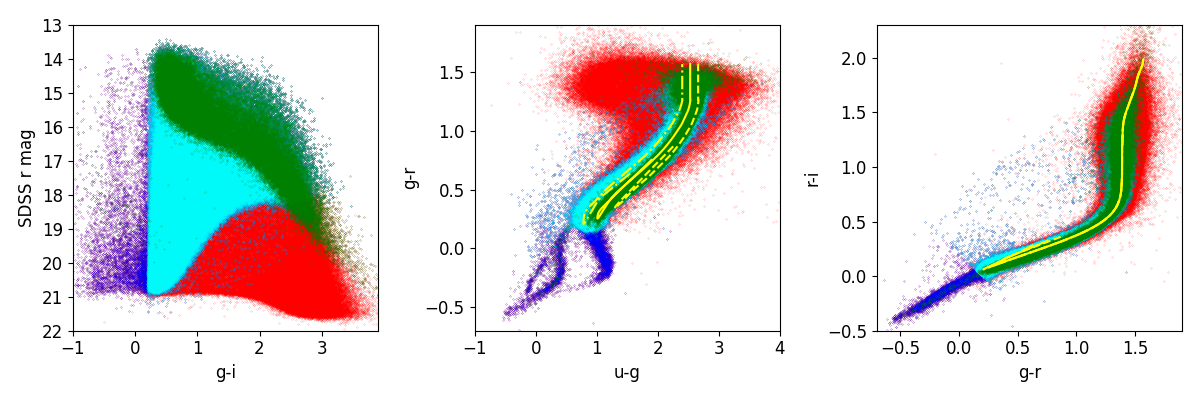
\includegraphics[width=1.0\textwidth,angle=0]{figures/plot3diagsData.png} 
\caption{An illustration of multiple stellar populations. The dots (of
any color) in the left panel show color-magnitude diagram for 841,000 stars from the SDSS Stripe 82 Standard Star Catalog
(variable sources are excluded, \citealt{2021MNRAS.505.5941T}) that have Gaia matches within 0.15 arcsec (after correcting for proper motion using Gaia measurements). A subset of 415,000 stars with $r < 22$ and $u<22$ are overplotted as blue dots, and 409,000 of those that also have $0.2 < g-i < 3.5$ (dominated by main-sequence stars and red giants) are overplotted as cyan dots. Finally, 63,000 stars that have signal-to-noise ratio for Gaia’s parallax measurements of at least 20 are shown as green dots (these stars can be used for the calibration of luminosity-color relations). The same symbol color scheme is used in other two panels. The three yellow lines in the middle panel show stellar locus parametrization used by Green et al. (2014) for three values of metallicity (left to right): $[Fe/H] = -2, -1, 0$. In the right panel, the impact of metallicity on color-color tracks is negligible and all three are indistinguishable from each other. In the bottom of the middle panel, at $-0.5 < g-r < 0$, the three dark blue sequences correspond to (from left to right) He white dwarfs, H white dwarfs, and blue horizontal branch stars. The clouds of pale blue dots visible above the main stellar locus in the middle and right panels correspond to unresolved binary stars \citep{2004ApJ...615L.141S}.} \label{fig:3dataDiags}
\end{figure*}



Our approach adopted here is essentially the same as used in recent papers\footnote{This approach greatly simplifies when studying
faint and distant blue halo stars, as in e.g., \cite{2008ApJ...673..864J}. Such stars are beyond the dust layer which is confined close
to the disk and thus $A_r$ can be obtained from IR maps, they have halo metallicities ($[Fe/H] \sim -1.5$), and can be assumed dominated
by main-sequence stars. As a result, a simple functional relationship, $M_r = f(g-i)$, or its generalized version that
accounts for the shift of $M_r$ as a function of metallicity \citep{2008ApJ...684..287I}, can be used to estimate distance
in a straightforward manner.}
by, e.g., \cite{2011MNRAS.411..435B},  \cite{2014ApJ...783..114G}, \cite{lallement_3d_2014}, 
\cite{gordon_panchromatic_2016}, \cite{queiroz_starhorse_2018}, \cite{green_3d_2019} and \cite{bailer-jones_estimating_2021}.
The main differences compared to these works include: 
\begin{enumerate}
\item The use of multiple stellar populations, in addition to main-sequence stars and red giants (white dwarfs, unresolved binary stars,
                blue horizontal branch stars; potentially Miras, quasars and RR Lyrae stars too, which can also be recognized and rejected using variability).
\item Improved color tracks for main-sequence stars and (especially) red giants, including the use of very young ($<$1 Gyr) populations 
               and an extended $[Fe/H]$ range. 
\item Priors based on sophisticated TRILEGAL simulations by \cite{2022ApJS..262...22D} that include multiple stellar populations and
               also account for the Galaxy's bulge component. 
\end{enumerate}
             
We discuss these improvements in detail in the next few sections. 


\subsection{Likelihood Computation}

Given a chosen model (i.e., a stellar population) $M$, the likelihood $p(D|M,\vec{\theta},I)$ can be explicitly written as
\begin{equation}
        \mathcal{L} \equiv p(D|M,\vec{\theta},I) = p(\vec{c}|M_r, [Fe/H], A_r).
\end{equation}
Assuming Gaussian photometric errors that are parametrized by a vector of color uncertainties $\vec{\sigma}$,
the log-likelihood is given by
\begin{equation}
   \label{eq:lnLcolors}
   \ln (\mathcal{L}) =  - {N \over 2} \, \ln(2\pi) - \sum_{i=1}^N \ln(\sigma_i) - {1 \over 2} \,\sum_{i=1}^N \left({ c^{obs}_i - c^{mod}_i  \over \sigma_i } \right)^2 \,
\end{equation}
where the summation is over all colors (for example, $N=4$ for SDSS, and $N=5$ for LSST), \ensuremath{c^{obs}_i} are the
observed colors and \ensuremath{c^{mod}_i} are the model colors (they are functions of $M_r$, $[Fe/H]$, and $A_r$
but for notational simplicity we don't explicitly list model parameters). Note that only the last sum involves model predictions
for colors ($c^{mod}_i$).

The model colors can be computed as
\begin{equation}
  \label{eq:reddCorr} 
                       \vec{c}^{\,\,mod}  = \vec{c}_0(M_r, [Fe/H]) + \vec{\delta c}(A_r),
\end{equation}
where $\vec{c_0}(M_r, [Fe/H])$ are intrinsic stellar colors for a given stellar population and $\vec{\delta c}(A_r)$ are
color corrections due to interstellar dust reddening. Eq.~\ref{eq:reddCorr} can be thought of as a set of 
3-dimensional data cubes, one for each color, that map the triplet ($M_r, [Fe/H], A_r$) to that color. 
The likelihood function can be thought of as a  3-dimensional data cube that, for a given set of observed colors $c^{obs}_i$,
maps the triplet ($M_r, [Fe/H], A_r$) to a 1-dimensional scalar, that is, $ln (\mathcal{L})$ is a scalar function of
$M_r$, $[Fe/H]$, and $A_r$.
        
The existence of multiple stellar populations in an SDSS photometric catalog is illustrated in Figure~\ref{fig:3dataDiags}.
With accurate multi-band photometry that includes a UV band (here SDSS $u$), main-sequence stars, red giants,
white dwarfs, blue horizontal branch (BHB) stars, and unresolved binary stars can be reliably identified (UV photometry
is also crucial for constraining metallicity). We discuss our choice of $\vec{c_0}(M_r, [Fe/H])$ for main-sequence stars
and red giants next, and then for white dwarfs, unresolved binary stars and BHB stars. 

\subsubsection{Empirical Luminosity-Color Tracks for Main-sequence Stars and Red Giants}

\begin{figure*}[b!]
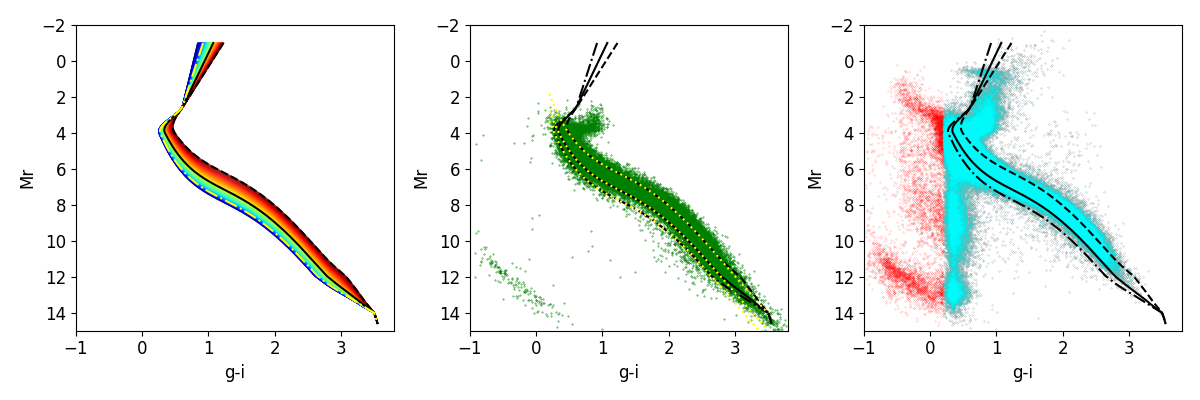
\includegraphics[width=1.0\textwidth,angle=0]{figures/plot3HRdiags.png}  
\caption{The left panel shows SDSS-based empirical absolute magnitude vs. color parametrization for main-sequence stars and red giants.
The data are color-coded by metallicity, ranging from $[Fe/H] = -2.5$ to 0 (blue to red). The three lines correspond to three values of
metallicity: $[Fe/H] = -2, -1, 0$ (dot-dashed, solid and dashed, respectively). The middle panel shows a sample of 63,000 stars that have
signal-to-noise ratio for Gaia’s parallax measurements of at least 20 (white dwarfs can be seen in the lower left corner.
Their absolute magnitudes are derived from parallax measurements. The dot-dashed,
solid and dashed black lines are the same as in the left panel. For comparison, the essentially identical yellow dotted lines were computed
using eqs. A2 and A7 from Ivezi\'{c} et al. (2008).  Note the discrepancy between these parametrizations and data for sub-giant stars ($M_r \sim 3-4$
and $g-i \sim 0.8-1.1$). The right panel shows a sample of 415,000 stars with $r < 22$ and $u<22$ as red dots (shown by blue dots in
Figure~\ref{fig:3dataDiags}), and 409,000 of those that also have  $0.2 < g-i < 3.5$ as cyan dots. Their absolute magnitudes were computed
using the so-called “photogeometric” distances from Bailer-Jones et al. (2021). The dot-dashed, solid and dashed black lines are the
same as in the left and middle panels. About 10,000 outliers (about 2.5\% of the full
sample) seen at $g-i = 0.4$ and $Mr > 7$ are predominantly found at the faint end ($r>20$).}
\label{fig:3HRdiags}
\end{figure*}


Both \cite{2012ApJ...757..166B} and \cite{2014ApJ...783..114G} used empirical color tracks for main-sequence stars
and red giants (see the left panel in Figure~\ref{fig:3HRdiags}, modeled after Figure 1 in \citealt{2014ApJ...783..114G})
derived from SDSS data for globular clusters (for technical details, see
Appendix A in \citealt{2008ApJ...684..287I}). These color tracks suffer from three problems. First, as can be seen in Figure 11 from
\cite{2014ApJ...783..114G}, their predicted colors for sub-giant stars between main-sequence turn-off and red giant branch are too blue by
about 0.1--0.2 mag. Second, their metallicity grid does not extend to the $[Fe/H]>0$ range relevant for some disk stars. Finally, they
correspond to very old populations (older than a few Gyr) and cannot be used for stars younger than about 1-2 Gyr. 

We use a combination of SDSS and Gaia data to demonstrate the first problem. The middle panel in Figure~\ref{fig:3HRdiags} 
shows a clear discrepancy between SDSS-based empirical tracks and data for sub-giant stars, using parallax-based absolute
magnitudes. Nevertheless, it is noteworthy that
for main-sequence stars the agreement is excellent. Furthermore, the right panel in Figure~\ref{fig:3HRdiags} demonstrates
that SDSS-based photometric distances and Gaia-based ``photogeometric'' distances from \cite{bailer-jones_estimating_2021}
for main-sequence stars are on the ``same scale''.  We discuss these
distance scales in more detail in \S\ref{sec:SDSSGaia}. 
 
We address all three problems by augmenting the SDSS-based empirical isochrones that correspond to old
populations with model-based isochrones that span a range of ages and a wider range of metallicities, which
results in better agreement with the observations. 
 

\subsubsection{Model-based Isochrones for Main-sequence Stars and Red Giants} 
 

\begin{figure*}[ht!]
\plotone{compare2isochrones_augmentedSDSS_1Gyr_10Gyr.png}
\caption{Augmented SDSS color tracks for two isochrone ages (left: 1 Gyr; right: 10 Gyr) and the full metallicity range
  ($-2.5 < [Fe/H] < +0.5$, color-coded linearly from blue to red). The black dots show the same sample of 63,000 stars from the middle panel in
  Figure~\ref{fig:3HRdiags}. As can be seen in the top right panel, sub-giant stars that could not be fit with empirical
  SDSS-based tracks (see the middle panel in Figure~\ref{fig:3HRdiags}) can be explained with tracks for old stars and
  intermediate-range metallicity. The sharp feature protruding from the main locus in the middle two panels corresponds
  to most luminous and evolved high-metallicity stars. Note that diagrams in the bottom row, which do not include
  the $u$ band, show very little dependence on metallicity.}  
\label{fig:augmLocus}
\end{figure*}

\begin{figure*}[ht!]
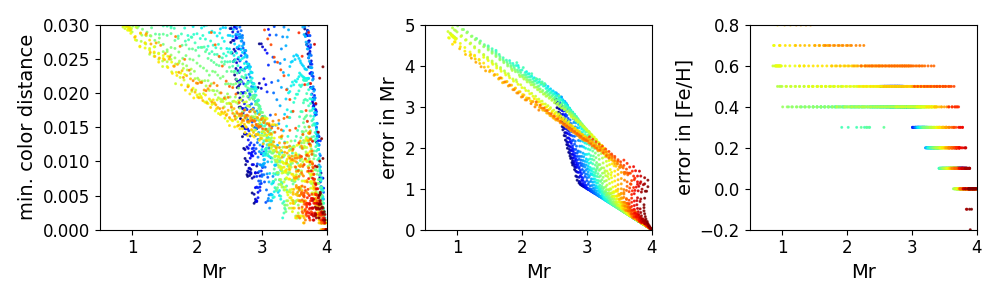
\includegraphics[width=1.0\textwidth,angle=0]{figures/RGdegeneracy.png}
\caption{Analysis of color degeneracies between giants and main  sequence stars. The left panel shows minimum color distance in
  4-dimensional color space ($u-g$, $g-r$, $r-i$, $i-z$) between a position on the locus with $M_r<4$ (giants) and any position on the
  main-sequence $M_r>4$ locus (in magnitudes). Symbols are color-coded by metallicity, linearly from blue to red for the range $-2.5$ to 0.5).
  The middle and right panels show errors in absolute magnitude and metallicity when a giant is misidentified as a main sequence star
  closest to it in color space.} 
\label{fig:RGdegeneracy}
\end{figure*}

We considered two sets of isochrones: the Dartmouth Stellar Evolution Database\footnote{See http://stellar.dartmouth.edu/models},
hereafter DSED \citep{2008ApJS..178...89D}, and PARSEC\footnote{http://stev.oapd.inaf.it/cgi-bin/cmd\_3.7} \citep{2012MNRAS.427..127B} isochrones. 
Both isochrone sets span adequate ranges of age and metallicity. Unfortunately, the computed color sequences show discrepancies
with the observed SDSS stellar locus at the level of 0.1-0.2 mag and cannot be used without further adjustments.

We ``augment'' the empirical SDSS-based isochrones in two steps:
\begin{enumerate}
\item We extend its metallicity range from $[Fe/H]=0$ to $[Fe/H]=+0.5$ by linear extrapolation of the color vs. metallicity
  dependence around $[Fe/H]=0$. We adjust the gradient by a multiplicative factor (0.7) to ensure that the bright end of the
  stellar locus at $[Fe/H]=+0.5$ agrees with SDSS-Gaia data (shown in the middle panel in Figure~\ref{fig:3HRdiags}).
\item 
  For $M_r < M_{TO}$, where turn-off absolute magnitude $M_{TO}$ depends on age and ranges from $M_{TO}$=4 for age = 1 Gyr
  to $M_{TO}$ = 5 for age = 10 Gyr, we ``attach'' model-based isochrones (we use DSED isochrones hereafter) to empirical
  SDSS-based isochrones.
\end{enumerate}

Examples of the resulting color tracks for two representative ages are shown in Figure~\ref{fig:augmLocus}. Sub-giant stars that could not
be fit with empirical SDSS-based tracks can now be explained with tracks for old stars and intermediate-range metallicity. 
We have computed such tracks for a grid of ages but believe that the two choices shown in Figure~\ref{fig:augmLocus}
(1 Gyr and 10 Gyr) should suffice for ``non-specialized'' bulk processing. The reason is that the locii for ages above 1-2 Gyr look
very similar to each other, while the fraction of stars younger than 1 Gyr is very small at the faint apparent magnitude
levels probed by SDSS and LSST. Of course, in sky regions with intensive star formation, a ``specialized'' approach with
a fine age grid can be easily executed.

We note strong degeneracies in color space between giants and main sequence stars (see Figure~\ref{fig:RGdegeneracy}). 
They are especially strong for sub-giant stars with $2 < M_r < 4$, for which it is always possible to find a matching main sequence star
closer in 4-dimensional color distance than 0.02 mag (and for $3 < M_r < 4$ even closer than 0.01 mag). Due to photometric scatter, 
such subgiant stars can be misidentified as a main sequence star and absolute magnitude errors can range up to several magnitudes.


These color tracks for main-sequence stars,  blue horizontal branch stars, and red giants account for an overwhelming majority of stars 
expected in SDSS and LSST catalogs (approximately $>$95\% but the fraction varies with apparent magnitude and sky position). 
Nevertheless, we also explicitly account for a few additional populations: white dwarfs and unresolved binary stars. 


\subsubsection{Luminosity-Color Tracks for White Dwarfs}

High-precision SDSS photometry clearly shows two white dwarf (WD) sequences in the $g-r$ vs. $u-g$ color-color diagram
(see, e.g., Figures 23 and 24 in \citealt{2007AJ....134..973I}, as well as the middle panel in Figure~\ref{fig:3dataDiags}).
A comparison with models from \cite{1995PASP..107.1047B}, as well as with SDSS spectra, reveals that the two sequences
correspond to H and He white dwarfs, with the mean log(g) = 8.0 for the H sequence and log(g) = 8.5 for the He sequence.
Upper limits for the scatter of log(g) around these mean sequences appear as no more than 0.5. 
We use three modern white dwarf catalogs: the Montreal White Dwarf
Database\footnote{https://www.montrealwhitedwarfdatabase.org} \citep{2017ASPC..509....3D}, the Gaia EDR3 White Dwarf Catalog\footnote{https://warwick.ac.uk/fac/sci/physics/research/astro/research/catalogues/} \citep{2021MNRAS.508.3877G}, 
and the Gaia-based White Dwarf Database\footnote{https://cdsarc.cds.unistra.fr/viz-bin/cat/J/A+A/679/A127} \citep{2023A&A...679A.127G}
to validate the \cite{1995PASP..107.1047B} models and derive small color offsets that bring models in perfect agreement with these three datasets.

We consider only white dwarfs with cataloged DA, DB or DC spectral class, at galactic latitudes further than 10 degrees from the plane,
with SDSS photometry, apparent magnitudes $5 \le m \le 22$ in any band $m$, and $15 \le r \le 19$, where $r$ is the SDSS $r$-band magnitude.
Observed magnitudes are corrected for interstellar dust extinction using maps from \cite{schlegel_maps_1998} and per-band extinction coefficients
discussed in \S\ref{sec:ismdust} below. We group the DB and DC spectral classes as He dwarfs (1,939 objects), while the DA spectral class corresponds
to H white dwarfs (9,307 objects). Their absolute magnitudes were calculated using ``photogeometric'' distances from \cite{bailer-jones_estimating_2021}. 

For each WD type (H and He) and SDSS color, we bin the data into 20 $M_r$ bins and compute the median value of a given color in each bin.
The color vs. $M_r$ sequences from \cite{1995PASP..107.1047B} are then slightly (up to 0.1 mag) shifted in color so that the mean offset for all bins
vanishes. The only case where a small (up to 0.1 mag) linear adjustment of the model track was needed is the $u-g$ color for H models at $g-r<-0.3$. 
After these color adjustments are applied, all color vs. $M_r$ model sequences were linearly interpolated to a common $M_r$ grid ($8.5 < M_r < 14.5$,
with a step of 0.02 mag). The resulting two model tracks for H and He white dwarfs are shown in Figure~\ref{fig:locusWDs}. 
   

\begin{figure*}[ht!] 
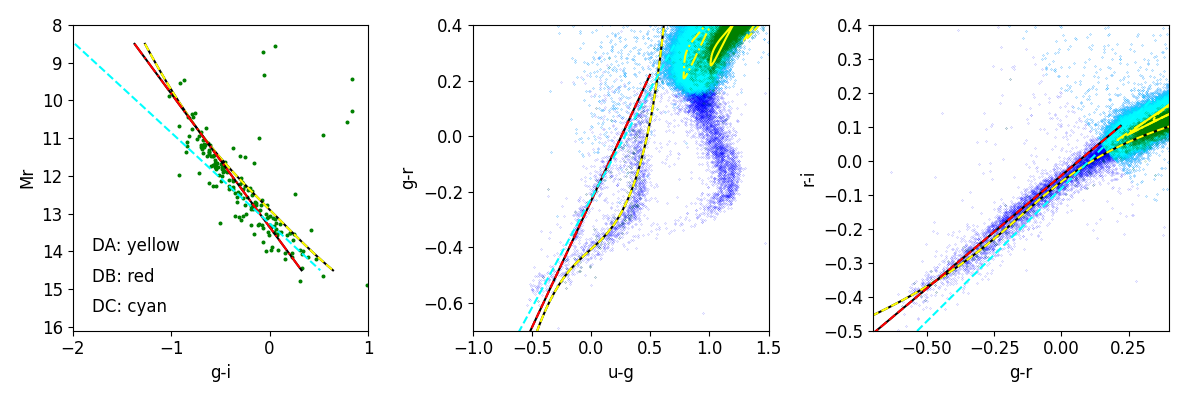
\includegraphics[width=1.0\textwidth,angle=0]{figures/plot3diagsBAzoom.png}
\caption{Luminosity-color tracks for H and He white dwarfs based on models from \cite{1995PASP..107.1047B}, with
  colors slightly shifted to bring them in agreement with SDSS photometry. Data, shown as symbols, are the same as in
  Figure~\ref{fig:3dataDiags} and in the middle panel in Figure~\ref{fig:3HRdiags}. Note the crucial role of the $u-g$ color
  for distinguishing H and He tracks.}
\label{fig:locusWDs}
\end{figure*}


\subsubsection{Luminosity-Color Tracks for Unresolved Binaries}

Following \cite{2004ApJ...615L.141S}, who discovered the so-called ``second stellar locus'' of unresolved binary
stars in SDSS dataset, we generate luminosity-color tracks for unresolved binaries consisting of an M dwarf and a white dwarf.
We limit models to M dwarfs because white dwarfs would have negligible impact on colors of more luminous main-sequence stars. 
M dwarfs are parametrized with $M_r$ and $[Fe/H]$, and H/He white dwarfs with $M_r$. Therefore, model tracks for unresolved binary
stars would have three model parameters. After numerical experimentation that revealed small model sensitivity to metallicity, we
decided to consider only M dwarfs with two metallicity values corresponding to mean metallicity for disk and halo populations:
$[Fe/H]=0$ and $[Fe/H]=-1.5$, respectively. For the remaining two model parameters, we selected $M_r$ corresponding to the
total system luminosity and the component luminosity ratio in the $r$ band. 

We sample the M dwarf luminosity in the range $8.5 \le M_r \le 14.5$, with a step of 0.1 mag, and for each value
generate a track by adding luminosity of a white dwarf, where the track is sampled on the same grid of $M_r$ but
using white dwarf models (separately for H and He models). There are four model families (for two families of white dwarf
models and two values of $[Fe/H]$ for M dwarfs), each with 3,721 $M_r$ vs. color entries. The color tracks for H white dwarfs
and $[Fe/H]=-1.5$ M dwarfs are shown in Figure~\ref{fig:locusBinaries}. Analogous tracks for binaries composed of an M dwarf with
$[Fe/H]=0$ and either an H or He white dwarf look very similar though not identical (differences are at most a few tenths
of a magnitude). In practice, it will be nearly impossible to constrain M dwarf metallicity, and very hard to distinguish
H and He white dwarfs. It may turn out that it will be sufficient to use a single model family to fit LSST data (e.g., a
combination of an H white dwarf and a $[Fe/H]=-1.5$ M dwarf). 



\begin{figure*}[ht!]
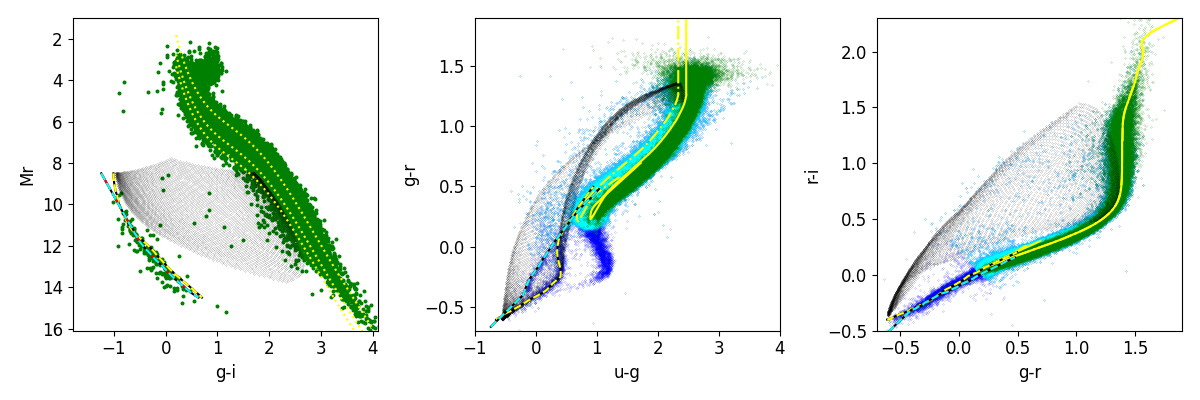
\includegraphics[width=1.0\textwidth,angle=0]{figures/plot3diagsBA_DAh.png}  
\caption{Luminosity-color tracks, shown with gray symbols, for unresolved binaries composed of an M dwarf with
  $[Fe/H]=-1.5$ and an H white dwarf. Analogous tracks for binaries composed of an M dwarf with
  $[Fe/H]=0$ and either an H or He white dwarf look very similar though not identical. Data, shown as colored symbols,
  are the same as in Figure~\ref{fig:3dataDiags} and in the middle panel in Figure~\ref{fig:3HRdiags}.} 
\label{fig:locusBinaries}
\end{figure*}

 


\subsubsection{Luminosity-Color Tracks for Unaccounted Populations}

There will always be sources that cannot be fully explained with any of the available families of
luminosity-color tracks. For example, quasars and RR Lyrae are not considered here
but can be easily recognized and removed from the sample in a straighforward manner since
they are variable \citep[e.g., see][]{2007AJ....134.2236S}. The remaining non-variable sources
that are not well fit with available models can be recognized as ``bad fits'' (see the last subsection on
model selection below). 

There will be impostors, too, with measured colors consistent with available model(s), but
with a very different nature (e.g., ultra-cold white dwarfs ``hiding'' in the main stellar locus).
As the time-domain information is built up with the progress of LSST, 
it might be possible to recognize them, for example, as high proper motion sources or perhaps
using a broader wavelength range through cross-correlation with other surveys (e.g., WISE or
Roman surveys). While they will require specialized studies, based on TRILEGAL simulations
we expect that their fraction in the sample should be very small (most likely $<1$\%). 


\subsubsection{Accounting for Interstellar Dust Extinction \label{sec:ismdust}} 

Given a stellar population and resulting color tracks for intrinsic un-extincted colors, colors need to
be corrected for interstellar dust extinction using an adequate dust extinction model. Additive color
corrections $\vec{\delta c}(A_r)$ (see eq.~\ref{eq:reddCorr}) can be computed as 
\begin{equation}
 \label{eq:extCorr} 
                      \delta c = (C_{m2}- C_{m1}) \, A_r,
\end{equation}
where $m1$ and $m2$ stand for two bandpasses that define the color (e.g., $u$ and $g$).  
Dust extinction models, such as \cite{1989ApJ...345..245C} and
\cite{1999PASP..111...63F}, parametrize extinction coefficients $C_{m}$ as functions of $R_V$, where
$R_V = A_V/E(B-V)$ and $E(B-V)$ is the stellar ``color excess'' \citep{1989ApJ...345..245C}.

Recent studies, such as \cite{2012ApJ...757..166B} based on SDSS data (including the Galactic plane), 
find that the scatter of $R_V$ around its mean value $R_V=3.1$ is very small. For this reason, we adopt
empirical results from their Table 1: $C_m$ = (1.810, 1.400, 0.759, 0.561) in $(u, g, i, z)$, respectively ($C_r=1$
by definition). This choice does not preclude the use of our framework to fit for $R_V$ as the fourth free
model parameter in Galactic plane regions with very large $A_r$ ($R_V$ is poorly constrained when $A_r$ is small);
we  can simply add multiple models with extincted colors generated using different values of $C_m$.

In our implementation, constraints on $A_r$ for two nearby stars, even if they have similar distances,
are independent. We note that one could use the so-called hierarchical Bayesian modeling  and specify the prior
for the line-of-sight extinction profile: nearby stars would then jointly constrain it. For more
details, see Green et al. (2014).

Finally, it is noteworthy to point out that the dust extinction vector is nearly parallel to the main stellar locus,
and this fact may cause model parameter degeneracies for certain choices of colors (e.g., see Figure~9 in
\citealt{2012ApJ...757..166B}). Such degeneracies are broken when multiple colors that span a wide
wavelength range and extend into near-IR (such as the $i-z$ color) are available. For more details, see
Section 2.8 in \cite{2012ApJ...757..166B}.


\subsection{TRILEGAL-based Priors \label{sec:priors}} 

\begin{figure*}[t!]
\hskip -0.5in
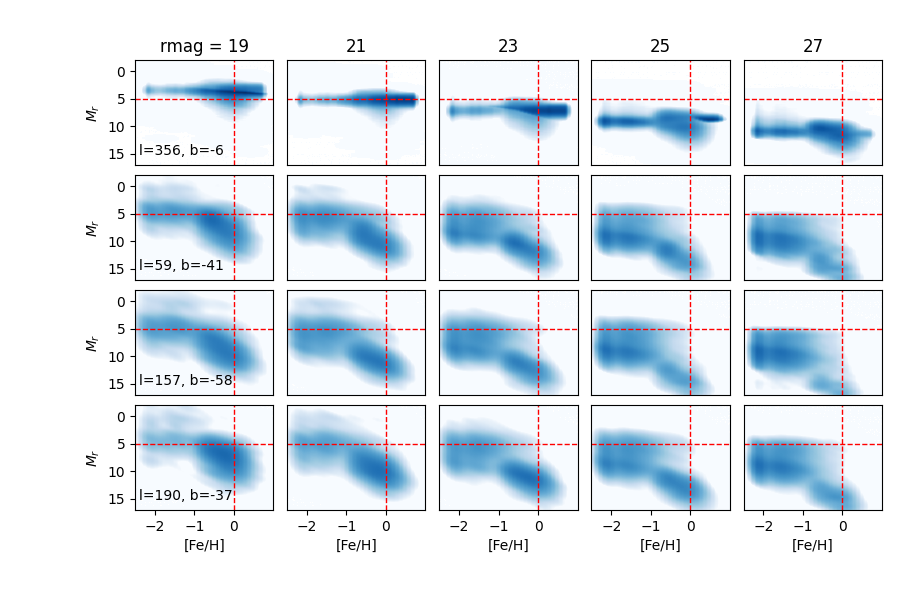
\includegraphics[width=1.07\textwidth,angle=0]{figures/Stripe82priorMosaic.png}
\vskip -0.4in  
\caption{Examples of priors for model parameters, $p(M_r, [Fe/H])$, for main-sequence stars and red giants,
  for four sky positions (rows, for locations see the first column) and for several brightness levels in the LSST
  magnitude range (left to right: bright to faint). The integral of each map over $M_r$ and $[Fe/H]$ is unity. 
  The dashed lines are the same in each panel and are added to guide the eye. 
}
\label{fig:priorsAstroLab}
\end{figure*}


In addition to specifying likelihood $p(\vec{c}|M_r, [Fe/H], A_r)$ for a given model $M$, we need to specify
the prior probability distribution for model parameters, $p(M_r, [Fe/H],A_r)$ (see eq.~\ref{eq:BayesPriorExpand};
we address the model probability $p(M|I)$ further below). First, we assume that the stellar model parameters
are unrelated to the distribution of interstellar dust along the line of sight,
\begin{equation}
 \label{eq:BayesPrior2}
               p(M_r, [Fe/H],A_r) = p(M_r, [Fe/H]) \, p(A_r).
\end{equation}
We adopt a uniform prior for $p(A_r)$ using the values $A_r^{SFD}$ taken from the \cite{schlegel_maps_1998}
dust extinction maps. To account for potential map errors, we set the maximum allowed value of $A_r$ as
\begin{equation}
          A_r^{max} =  a \, A_r^{SFD} \, + \, b,
\end{equation}
and $a=1.3$, $b=0.1$, where the choice of these parameters allows for plausible upper limits for additive and
multiplicative errors in the dust extinction maps. Therefore, $p(A_r) = 1/A_r^{max}$ for $0 \le A_r \le A_r^{max}$
and $p(A_r) = 0$ for $A_r > A_r^{max}$.  

The prior distribution of stellar model parameters, $p(M_r, [Fe/H])$, depends on sky position and apparent
magnitude (here $r$) due to the complex structure of the Milky Way. For example,  \cite{2014ApJ...783..114G}
generated priors using SDSS-based analytic descriptions of the 3-dimensional stellar distribution in the Milky Way
\citep{2008ApJ...673..864J} and metallicity distribution for disk and halo components \citep{2008ApJ...684..287I}. 
Since LSST aims to provide good coverage of the Galactic plane and the Bulge, where SDSS data did not provide strong
constraints, we opted to utilize recent simulations that implement constraints from a variety of modern surveys (some
include the Galactic plane and Bulge regions). 

\cite{dal_tio_simulating_2022} have generated a mock catalog of the Milky Way stars to LSST depth ($r$=27.5) and over
the entire LSST survey area. The simulation is based on the TRILEGAL code, incorporates all principal stellar populations,
includes about 10 billion stars, and the catalog is publicly accessible through the NOIRLab Astro Data
Lab\footnote{Available at https://datalab.noirlab.edu/}.
We have developed code to query this mock LSST catalog using Astro Data Lab portal. For a given position on the sky, we
extract all catalog entries from an area of $\sim$10 deg$^2$ (the size of the LSST Camera's field of view) around it, then bin
the sample by apparent $r$-band magnitude (27 bin centers from $r=14$ to $r=27$, with a bin width of 1 mag). 
Given an $r$-band selected subsample, we separate all modeled populations and then bin them using adequate model
parameters (e.g., $M_r$ and $[Fe/H]$ in the case of main-sequence stars and red giants). The resulting 2-dimensional map
is renormalized so that its integral over all model parameters is unity.

Figure~\ref{fig:priorsAstroLab} shows examples of such $p(M_r, [Fe/H])$ maps for a grid of apparent magnitudes and for
several characteristic sky positions. Several features are noticeable: i) there are two ``clouds'', at low and high metallicity,
that correspond to halo and disk stars; ii) the distribution towards the Galactic center (top row) is much more compact in
the $M_r$ direction (because these subsamples are dominated by the Bulge stars at similar distances); iii) the whole 
distribution shifts to fainter levels as the bin center ($r$) becomes fainter. We have experimented with different region
sizes\footnote{We use HEALPix geometry, see https://healpix.jpl.nasa.gov.} and found that $\sim$10 deg$^2$
(HEALPix $N_{side}$=16 and 32, with 3,072 and 12,288 pixels over the full sky) is sufficiently small to capture the
variation of $p(M_r, [Fe/H])$ maps across the sky.
 
 
\subsection{An Example of Bayesian Model Parameter Estimation}


\begin{figure*}[t!]
\hskip -0.7in
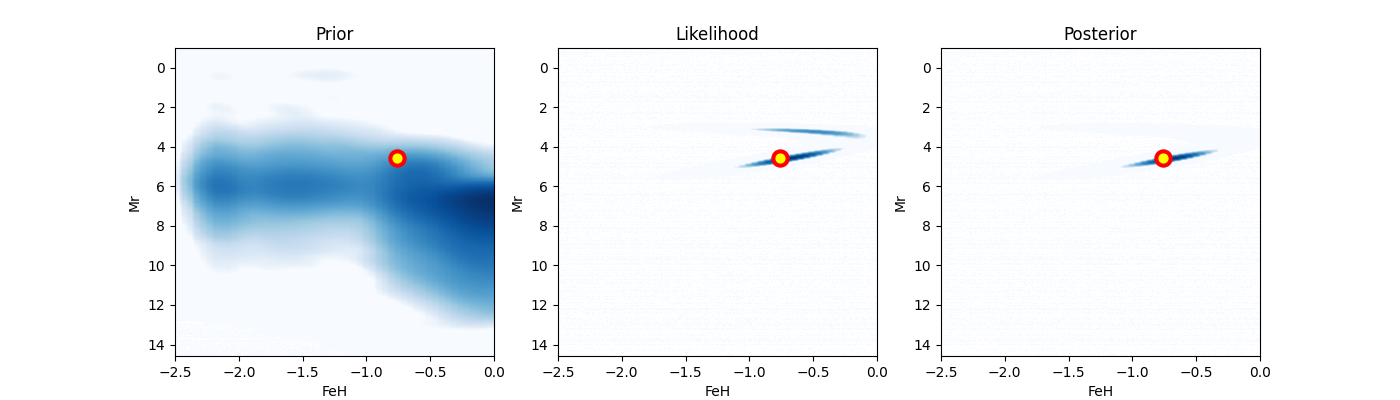
\includegraphics[width=1.2\textwidth,angle=0]{figures/bayesPanels_ex1.png}
\caption{Maps of the prior (left), likelihood (middle; computed using eq.~\ref{eq:lnLcolors}) and posterior (right;
computed using eq.~\ref{eq:BayesFull}) for a simulated main-sequence star with $r=21.2$, $(g-r)=0.48$,
$M_r= 4.58$, $[Fe/H]=-0.76$ and $A_r=0.37$. The prior in the $A_r$ direction is uniform. The circles mark
the values of input $M_r$ and $[Fe/H]$. The posterior marginal distributions for all three model parameters
are shown in Figure~\ref{fig:cornerPlot3ex1}.
}
\label{fig:bayesPanels}
\end{figure*}
 
We use isochrones shown in the right panels of Figure~\ref{fig:augmLocus} and priors shown
in the second row of Figure~\ref{fig:priorsAstroLab} to illustrate the Bayesian model parameter estimation. 
Figure~\ref{fig:bayesPanels} shows prior, likelihood and posterior for a main-sequence star close to the
turn-off point. Note how the posterior, although much wider than the likelihood map, helps break the
degeneracy\footnote{Priors can break degeneracies between the giant and dwarf stars because luminous
stars become strongly disfavored at faint magnitudes (because an apparently faint giant star would imply
a very large distance, beyond the presumed edge of the Galaxy at $\sim$100 kpc; for example a giant star
with $M_r$=0 and $r$=22 would imply a distance of $\sim$250 kpc).} in the likelihood map (the two ``islands'').


\begin{figure}[t!]
  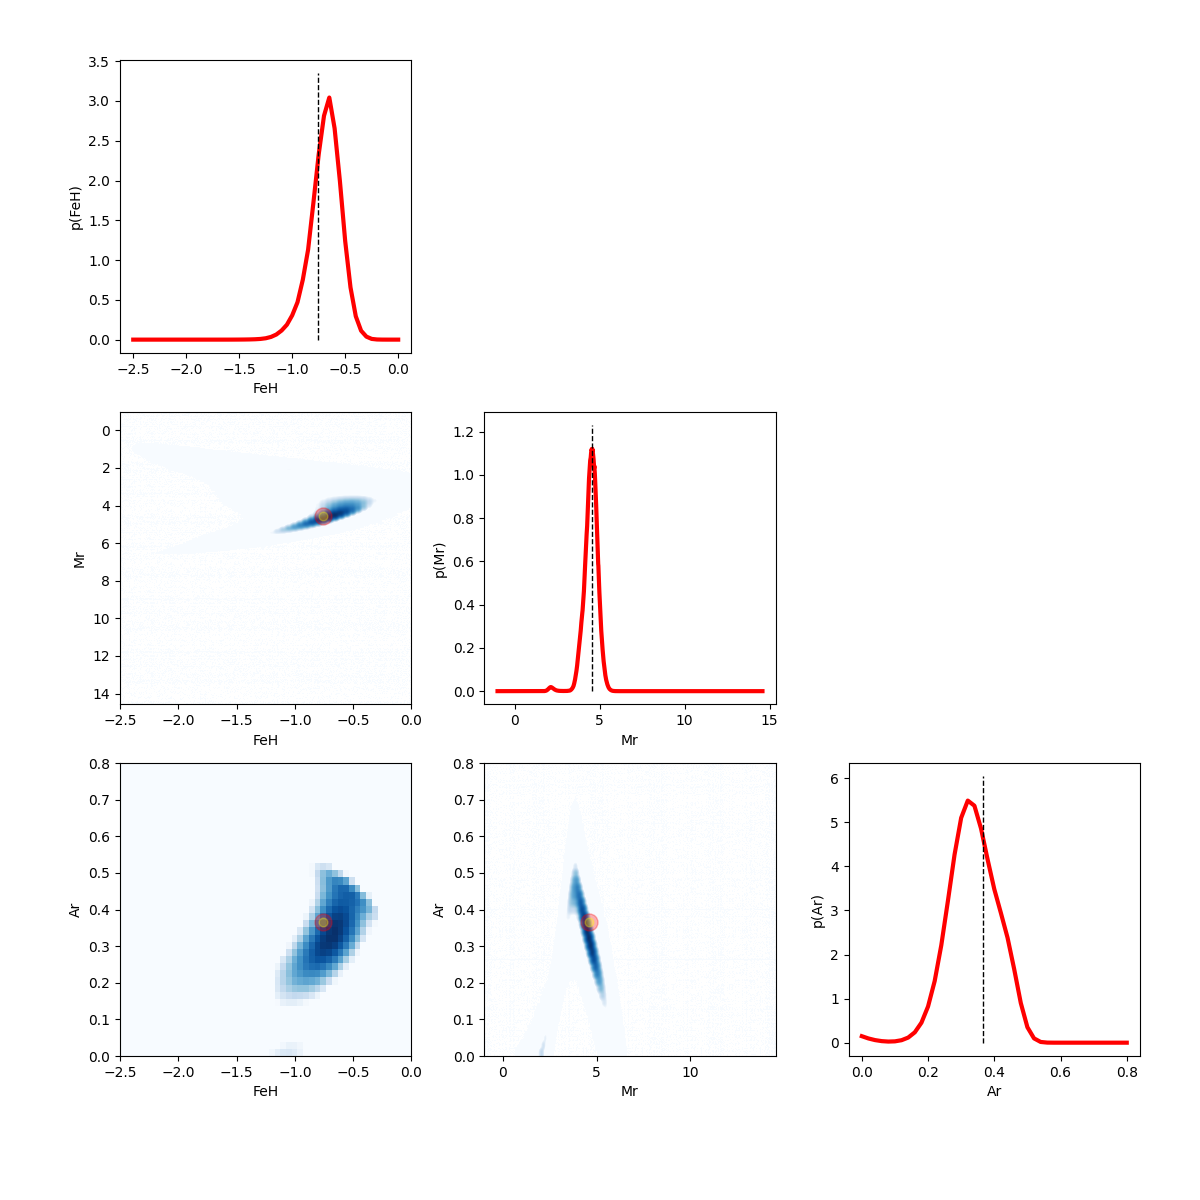
\includegraphics[width=1.0\textwidth,angle=0]{figures/cornerPlot3_ex1.png}
  \vskip -0.5in
\caption{Two-parameter covariances and marginal distributions for
  the posterior map from Figure~\ref{fig:bayesPanels}. The symbols and
  dashed lines show true input values.}
\label{fig:cornerPlot3ex1}
\end{figure}


Figure~\ref{fig:cornerPlot3ex1} shows two-parameter covariances and marginal distributions for this case.
Note that true values are recovered within expected uncertainties, as well as non-vanishing covariances
between the parameters. The marginal distributions produced with the prior, likelihood and posterior maps,
shown in
% Figure~\ref{fig:margPost3D},   % FOR SOME REASON, THIS REFERENCE DOESN'T WORK
Figure 9,
illustrate the improvement in the ``knowledge'' of model
parameters between prior and posterior, brought by color measurements via the likelihood map. 


% 3D Bayes results for star i= 1
% r mag: 21.19 g-r: 0.481 chi2min: 2.7487013195215177
% Mr: true= 4.58 estimate= 4.49193855789433  +-  0.418936340852099
% FeH: true= -0.76 estimate= -0.6860134814469806  +-  0.14586005018974993
% Ar: true= 0.367 estimate= 0.3349289555609109  +-  0.07573177303312867
% Qr: true= 4.947 estimate= 4.831891055998594  +-  0.38018147434019617


\begin{figure}[t!]
%\plotone{margPosteriors3D_ex1.png}
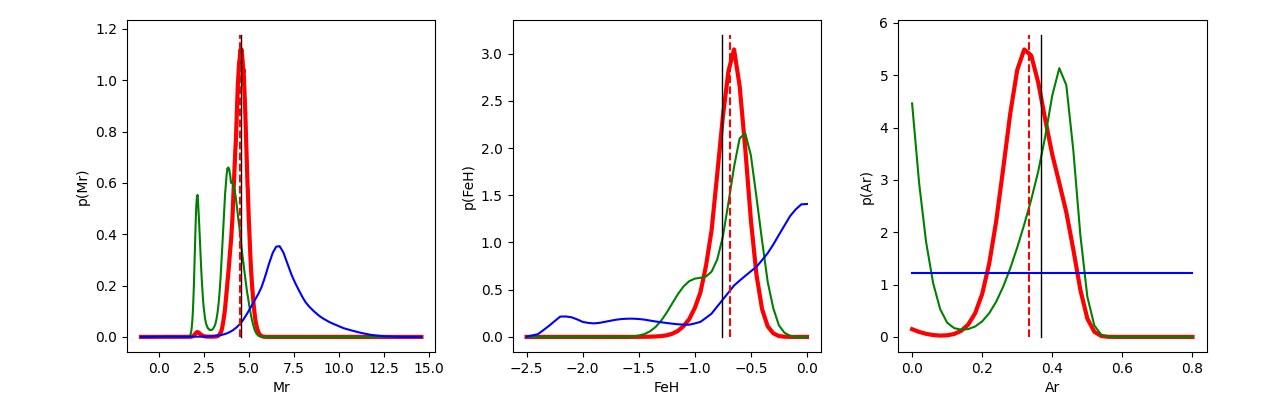
\includegraphics[width=0.99\textwidth,angle=0]{figures/margPosteriors3D_ex1.png}
\caption{An illustration of the improvement in the ``knowledge'' of model parameters between prior and posterior,
brought by measurements via the likelihood map. The lines show marginal distributions produced with the
prior (blue), likelihood (green) and posterior (red) maps from Figure~\ref{fig:bayesPanels}. The dashed line shows the
expectation value for the marginalized posterior and the vertical solid line marks the true input value.}
\label{fig:margPost3D}
\end{figure}



In the next Section, we discuss a fast numerical pipeline implementation that can perform this computation for LSST-sized
catalogs and provide a more quantitative analysis of the method's performance.  We conclude this Section with a brief
discussion of Bayesian model selection method for assigning posterior probabilities to each stellar population used to interpret
observations. 


\subsection{Bayesian Model Selection \label{sec:ModSel}} 

For each star and for each stellar population (that is, a model for color-magnitude tracks), a posterior
3-dimensional data cube is produced.  These posteriors are used when choosing the best model, as follows.

Bayes' theorem as introduced by eq.~\ref{eq:BayesFull} quantifies the posterior
pdf of parameters describing a single model, with that model {\it assumed to be true}.
To find out which of two models, say $M_1$ and $M_2$, is better supported by data, we
compare their posterior probabilities via the {\it odds ratio} in favor of model $M_2$ over
model $M_1$ as 
\begin{equation}
                  O_{21} \equiv { p(M_2|D,I) \over p(M_1|D,I) }.
\end{equation}     

The posterior probability for model $M$ ($M_1$ or $M_2$) given data $D$, $p(M|D,I)$  in this
expression, can be obtained from the posterior pdf $p(M,\vec{\theta}|D,I)$ in eq.~\ref{eq:BayesFull}
using marginalization (integration) over the model parameter space spanned by $\vec{\theta}$.
The posterior probability that the model $M$ is correct given data $D$ (a number between 0~and~1)
can be derived using eqs.~\ref{eq:BayesFull} and \ref{eq:BayesPriorExpand} as
\begin{equation}
             p(M|D,I) =  {p(D|M,I) \, p(M|I) \over p(D|I)},
\end{equation}           
where
\begin{equation}
\label{eq:evidence}
       E(M) \equiv p(D|M,I) = \int p(D|M,\vec{\theta},I) \, p(\vec{\theta}|M,I) \, d \vec{\theta}
\end{equation}
     
is called the {\it marginal likelihood} (or {\it the evidence}) for model $M$ and it quantifies the 
probability that the data $D$ would be observed {\it if} the model $M$ were the correct model.
Since the marginal likelihood $E(M)$ involves integration of the data likelihood $p(D|M,\vec{\theta},I)$,
it is also called the {\it global likelihood} for model $M$.

The global likelihood is a {\it weighted average} of the likelihood function, with the prior for model parameters
acting as the weighting function. Alternatively, $E(M)$ is simply the integral over allowed parameter space of
the posterior pdf before its renormalization to set this integral to unity (e.g., the integral of the posterior shown
in the right panel in Figure~\ref{fig:bayesPanels}). If the chosen model color tracks cannot explain the observed
colors, the likelihood (eq.~\ref{eq:lnLcolors}) will never be very high and the resulting $E(M)$ will be low.
We note that in the limit of Gaussian posterior and flat priors, Bayesian evidence-based model selection becomes
equivalent to $\chi^2$ selection from the frequentist statistical framework. 

The probability of data, $p(D|I)$, cancels out when the odds ratio is considered: 
\begin{equation}
       O_{21} =  {E(M_2) \, p(M_2|I) \over E(M_1) \, p(M_1|I)} =
       B_{21} \, {p(M_2|I) \over p(M_1|I)}. 
\end{equation}
In practice, the values of the odds ratio are interpreted using Jeffreys' scale (see, e.g., Chapter 5 in \citealt{2020sdmm.book.....I});
in particular, $O_{21}>10$ represents ``strong'' evidence in favor of $M_2$ ($M_2$ is ten times more probable than $M_1$).
     
The ratio of global likelihoods, $B_{21}\equiv E(M_2)/E(M_1)$, is called the {\it Bayes factor}, and
is equal to 
\begin{equation}
     B_{21} = {\int p(D|M_2,\vec{\theta}_2,I) \, p(\vec{\theta}_2|M_2,I) \, d \vec{\theta}_2 \over
                    \int p(D|M_1,\vec{\theta}_1,I) \, p(\vec{\theta}_1|M_1,I) \, d \vec{\theta}_1}.
\end{equation}
The vectors of parameters, $\vec{\theta_1}$ and $\vec{\theta_2}$, are explicitly indexed to emphasize
that the two models may span vastly different parameter spaces (including the  number of
parameters per model).

The prior model probabilities, $p(M_1|I)$ and $p(M_2|I)$, are determined using TRILEGAL simulated catalog.
For example, if model 1 is main-sequence stars and model 2 is white dwarfs, we estimate the $p(M_2|I)/p(M_1|I)$
ratio by simply counting main-sequence stars and white dwarfs in the corresponding $r$ magnitude bin. 

In case of $N_M$ models, we assume that they represent an exhaustive model set and estimate the posterior
probability of model $k$, $k=1...N_M$, as
\begin{equation}
                 p(k) = { O_{k1}  \over \sum_{j=1}^{j=N_M}  O_{kj}},
\end{equation}
where the model $k=1$ is chosen arbitrarily without a loss of generality ($O_{11}$ = 1).
% We will illustrate model selection with multiple stellar populations in the next Section.



